The purpose is to discuss what came out of the wind power and electricity price results from the experimental results. The results will be compared to each other but also related to literature.
\todo{compare trimming in more detail}
\todo{discuss reconfigurability of the system when used in real life setting}

\subsection{Experiment one}
\label{sec:inputParameterDiscussion}
\subsubsection{Identifying input parameters}
The strength of the prediction is very much dependent on the quality of the underlying data. As described in Section~\ref{sec:dataCollection} the data must satisfy certain criteria before it can be used as input and output for the Artificial Neural Network. It must be trustworthy and contain hourly observations for our specific purposes, e.g. day-ahead wind power and electricity price prediction based on a dataset that consists of hourly observations. All calculations in the ANN are based on this data which makes it of utmost importance for the forecast. The selection of the correct input parameters for testing is equally important which is described in the analysis in Chapter~\ref{ch:theANNs}. The analysis of both electricity price and wind production together with experiment one in Sections~\ref{sec:windPowerExperimentOne} and~\ref{sec:priceExperimentOne} show how the combination of the right parameters is the core to a good prediction. It is necessary to make a comprehensive analysis of different parameters to know what to include in the experiment and how to represent them. A good example of this is the seasonal aspect for electricity prices which showed difference in result when used as month or as the specific season (summer, winter, ect.). Consequently, the pre-requisites for the wind power and electricity price experiments to perform accurately is the the quality and selection of the input data since it is the basic foundation for the Artificial Neural Network to generalize upon. 

\todo{Core parameters in wind power is more clear than for price. Wind will always have the same influence on the wind mills no matter the place whereas price is much more dependent on the underlying market forces --- this is seen from the result but also in the co-relation between wind speed and wind power}

Examples of publications where the importance of analysing exactly what input parameters constitutes the electricity price, why and how they are represented is limited is in\cite{szkuta1999electricity,sansom1999neural,1} which is also discussed in Section~\ref{sec:priceExperimentThree}. A sensitivity test to identify influences have been carried out for 4 out of the 15 input in \citep{szkuta1999electricity} and there is no description of the last parameters. Article \cite{1} decided only to use only historical price data for prediction but without going into detail how it is represented. It makes it very difficult to imitate the behaviour and use or test their knowledge and experience on how to include and represent inputs in the best possible way. The seasonal aspect can as mentioned be included in different ways, matrix can be used and the combination of the inputs have very different impact. Exactly what combination of inputs and how they are represented should always be documented for others to imitate and test on own datasets so that results can be compared based on the same data. Our experiments showed that even though some inputs was closely co-related to the output it was not necessarily included in the best prediction as seen with consumption and wind power in Section~\ref{sec:windPowerExperimentOne}. The black box nature of the ANN can identify unforeseen dependencies between the various input parameters. It is not enough to simply list the characteristics of the output to predict without mentioning what came out of the input analysis, did the experiments validate it and exactly what inputs was used. The analysis is the foundation for what the experiments are suppose to validate, e.g. the various hypothesis's of experiment one are build based on the analysis. Expectations that was not met can also be explained by the analysis, for instance the substitution of consumption with air density or temperature. What influence the electricity price can differ from country to country due to different market conditions and different weather which makes it necessary to include it. In \cite{sansom1999neural} the input analysis is described with the following statement:

\begin{quotation}
\textit{The 13 inputs to the neural network were selected by data analysis and by trial and error to produce the seven-day ahead electricity price forecast. The inputs were time, demand and price data obtained from the SEM web site...}
\end{quotation}

The focus should not be on the results alone but also how the result is obtained through the dataset, especially in the case of input parameters for the neural network which have shown to be of utmost importance in our analysis. The point being that all publications use different datasets and experimental environments and in order to compare results to one another the different settings must be the same and tested on the same dataset. The lack in description of test environment and input analysis makes such comparisons difficult both due to the incomplete information but also because the format of the datasets can't be seen or downloaded to extract the information from yourself. Comparison with another publication was attempted in Section~\ref{sec:priceExperimentThree} and it showed the difficulties in comparing because we can never be certain of their experimental setup without it being properly documented --- it can be discussed if is even fair. The purpose of our thesis is amongst other things to identify the feasibility of an Artificial Neural Network used for prediction of wind power and electricity prices. The above discussion is related to this topic because the feasibility of the ANN is directly dependent on the quality and transparency of the data that it generalizes upon. The analysis that identifies the correct inputs together with the experiments to verify the best combination and network configuration is the foundation for the result and in our experience the most time-consuming, e.g. the actual analysis and how to get from there to the best possible network setting.

\subsubsection{Input combination}
As described above the different combinations of input parameters is found in experiment one for both electricity prices and wind power production. The experiments show the complexity in the black box nature of ANN since it identifies better connections of input than foreseen. In wind power production the substitution of temperature and air density with consumption showed better accuracy which was not expected, whereas wind speed showed to be much more crucial to the electricity price than foreseen. Wind power production impacts the electricity price as presented in \cite{dayAheadImpactOfWindPowerForecasts} but more than expected through the wind speed. This leads to the potential of feeding the electricity price with the prediction of wind power as input instead of wind speed to make the prediction more accurate. This connection has to be investigated in future work.

The seasonality characteristic of the wind power production and electricity price time-series is in both cases significant and for that reason expected to increase performance for both predictions. Seasonality is reflected in the month input parameter and showed different results. The month parameter obviously decreased the overall performance of the network in the case of wind power whereas it was increased in the electricity price. The first thought was the small size of the data only containing three months and therefore not reflecting the the seasons from the previous year which was the intention. When attempted on a whole years training set it showed an overall worsening in accuracy due to over-training due to the bigger training set. The electricity prices with the seasonal aspect was also tried with a training set containing a year but as opposed to wind power the accuracy of the forecasts stayed the same. What can be concluded from this is that more data is not necessarily equal to better results in both cases and 3 months of data is the most expressive to predict 24 hours ahead in our case. What was believed to be problematic was the shifting from one season to another where the new season was significantly different from the one we came from. This was proven wrong by the experiments since 3 months itself showed to contain enough information about the current season to be accurate and the the potential shortcomings from seasonal shifts were compensated by the omission of unnecessary data from the rest of the year. The high volatility results in many different cases during the year which can make it hard for the network to generalize when the data set becomes to huge.

\subsubsection{Unseen data}
\label{sec:unseenDataDiscussion}
The wind power section emphasized in connection with input parameter experiments the need for measuring accuracy of results only on the testing set (unseen data). It was seen in Table~\ref{table:predictionMAEUnseenVsTrainingSet} that the MAE could be the same across all predictions on the training set compared to a huge difference when applied on the testing set. The best MAE on unseen data showed the worst MAE on the training set. Furthermore, different seasons and consumptions during the year result in many different days where the electricity prices and wind power behaves differently. This is also discussed in the analysis in Chapter~\ref{ch:theANNs} and therefore the experiments must as a minimum be performed on an entire year of unseen data to cover all possible scenarios and thereby reflect reality. All simulations in this thesis is performed once on a year but more testing on the same year could be conducted to further validate and strengthen results. This stands opposed to the 5 weeks from different seasons used in \cite{1} which is argued to ensure fairness in results and reflect reality. A last example is in \cite{pjmForecast} where the experiments are performed on 5 different days throughout an entire year and then again on 2 weeks in February. Based on these days they conclude the following:

\begin{quotation}
\textit{The test results obtained through the simulation demonstrate that the proposed algorithm is robust, efficient, and accurate, and it produces better results for any day of the week.}
\end{quotation}

Omitting 340 days and concluding that it in general obtains better results is in contrast with our analysis of the seasonal aspect because they days differ much but also the results from experiment five in Section~\ref{sec:windPowerExperimentFive} and~\ref{sec:priceExperimentFive} where various starting points during the year greatly influences the overall results. The same omitting of testing days applies for~\ref{yamin2004adaptive} where a fixed testing period of one week is used for all experiments and at the same time basis for their conclusion. According to our experiments a more comprehensive testing period must be taken into consideration due to the different days and different results when claiming the feasibility and sufficiency of the prediction. One point to bring forward from~\ref{yamin2004adaptive} is the discussion of the use of Monte Carlo to eliminate randomness by running the same experiments more than once. The ANN can give somewhat different results even though predicting the same days due to the weights being initialized randomly every time. The suggested method could be used in our experiments to strengthen the results but it could result in time becoming an issue due to the huge amount of tests already conducted. The way we try to eliminate randomness is by predicting an entire year so that all seasons are represented but at the same reducing it by predicting many similar days many times during the whole year. Running the experiments more than once could be incorporated in such a way that an amount of the best predictions in every experiment could be run several times to ensure the results, for instance top-10.


\subsection{Experiment two}
\label{sec:matrixTrimmingDiscussion}
Dataset manipulation and trimming of the dataset are two important techniques that can improve the predictions of an artificial neural network.
\subsection{Matrix}
We used a matrix representation (described in Section~\ref{sec:Matrix}) for the input parameters that were applicable for such a representation. The input (applicable for matrix) has to have a finite and limited set of values and a significant difference in the influence on the output between the values. The inspiration for the matrix representation came from the way pictures are represented in ANNs. In \cite{knerr1992handwritten} they take every pixel (which has 16 different shades of grey) in a 16 pixel big image and map the pixels out as a matrix. This gives them 256 input variables for the neural network to represent this image. We do the same thing for the applicable input parameters but instead of pixels we map out values.

The matrix format has limitations (as we saw in the wind power experiment two in Section~\ref{sec:windProdExperimentTwo}). The input parameters you want to represent as a matrix has to be evenly distributed in the dataset e.g. time of day, day of week etc. If this is not the case; some of the input values might be under trained(from under representation) and lead to errors in the predictions instead of improvements. This was the case with wind speed as a matrix and the reason to why it was worse than the wind speed as a single input variable. When we applied the matrix format to the time of day input variable we saw an improvement in both cases. We did a simple matrix test in the wind speed experiment two (Section~\ref{sec:windProdExperimentTwo}) as we only had two different parameters that were applicable for the matrix format and because we saw that the wind speed as a matrix did perform poorly. In the price experiments we did a more elaborate test of the matrix format and did every combination (all with matrix, all without matrix and mixed). We did those because the price experiments had more parameters that was representable on the matrix format thus giving us more combinations. The results from the price experiment was not as lopsided regarding the matrix format as the wind production experiments. In the price experiments we could not say that one parameter had to be on one specific format but the combinations of the inputs both as matrix and non-matrix proved to be the best - we saw that the matrix format was overrepresented in the top results giving us a hint about it being the better choice.

We have only seen one other \cite{crowley2005weather} use the matrix format (to some extend) for their seasonal inputs. They represented their days in the week as a matrix format. They do not argue why they did it like that but we can see that they did it in their table of inputs. At the same time they do not evaluate the results compared to non-matrix representation. The following articles has seasonal inputs but do not utilize the matrix format \cite{szkuta1999electricity, singhal2011electricity} or at least do not disseminate it. If they actually do represent their seasonal inputs as matrices they should write it. This follows our thoughts about transparency and reproducibility we argued for in \ref{sec:unseenDataDiscussion}.

\subsection{Trimming}
Trimming of the dataset is a technique to remove irregularities in the dataset. This can be done both for the highest values and the lowest values in the dataset. Trimming allows us to get a more standardized dataset but it comes at a cost. All the data that you remove from the dataset you will not be able to predict in the test dataset thus introducing limitations to the predictions. Therefore trimming should always be weighed up against how much of the dataset you will not be able to predict after the trimming. If the irregularities are extreme enough and under-represented in the dataset then we will not be able to predict these values (because of under-training towards these extremes). If this is the case the outliers just introduce errors and do not add benefits thus justifying the removal of these values.

In the wind power predictions experiment two (Section~\ref{sec:windProdExperimentTwo}) there was no benefit from trimming the dataset. Actually it introduced errors and made the predictions worse in average. This is because the dataset used for wind power production already consists of uniform dataset and the trimming will only scramble this data and introduce further volatility (described in Section~\ref{sec:windProdExperimentTwo} and shown in Figure~\ref{fig:fivePercentTrimPrediction}) because of this we will only focus on price in this section. In the electricity price prediction experiment two (Section~\ref{sec:priceExperimentTwo}) we saw that the trimming helped the predictions to be better. This is because in the price prediction dataset there were some extreme outliers. When we trimmed the dataset by 1\% in the top we went from 1561 to 632 as the highest value in the dataset. The 1\% we removed from the dataset only introduced more noise and was not predictable thus removing them did not make the performance worse - instead it helped the remainder of the results see Figure~\ref{fig:1PTrim}. We saw an improvement of 20,99\% from a non-trimmed dataset compared to a trimmed dataset (in the price predictions).

In \cite{singhal2011electricity, yamin2004adaptive} they also trim the dataset when predicting the electricity prices to get rid of the worst spikes in the price. In \cite{yamin2004adaptive} describe detailed how they use trimming in their dataset. They use a form of trimming called Winsorising\cite{Winsorising} where they instead of removing the data(trimming) they just set the values of the outliers to a specific value. In their case they set the upper value to \$50 and set everything above that to \$50. The interesting part is that they introduce a post-processing scheme where they revert the Winsorising after the predictions thus not removing the high values from the set but just limiting the negative effects of outliers. If this was done on our dataset we would see a decrease in performance\cite{yamin2004adaptive} but we would have a more accurate measure for how it would perform on live data. We see this as future work to test if this method would work on our dataset. Both matrix and trimming shows the need for preprocessing of the dataset also stated in \cite{yamin2004adaptive}. Preprocessing is important but it is also very important to communicate it to the reader of the paper due to the significant improvements in the performance. In \cite{sansom1999neural, 1} they do not mention anything about spike prices or whether they account for it. This might be because their dataset does not contain any spikes which (especially in large datasets) seems implausible see section about price volatility \ref{sec:volatility}. Which means we would have a hard time recreating their experiments and see how well it performs on our dataset.

Another obstacle when talking about trimming is how it can be applied on a live dataset. Since we do not know what the price is for the next 24 hours we will not be able to include this in our calculations regarding what should be trimmed and what should not. If we chose to apply trimming we can only do those calculations on the training set. As mentioned earlier this makes us unable to reproduce the values that has been removed from the dataset. If the system was to be used in a real live setting as a decision support system the aforementioned limitations and what is written in \ref{sec:uncertainInformation} really emphasizes how important transparency is. We need to make the user aware of the limitations and benefits of trimming thus giving them an informed choice to make.

\todo{Skriv om den her i forhold til pjmForecast}

\subsection{Experiment three}
\label{sec:calculatedInputDiscussion}
\subsection{Influence of trend}
\label{sec:influenceOfTrendInCalcInput}
Calculated inputs showed very different results. The electricity price prediction showed an overall improvement when adding slope, skewness and volatility as input. The alternative scatter approach from \cite{singhal2011electricity} where previous hours are directly added as inputs for the network to calculate the relationship itself was outperformed by the direct input calculations. Skewness and volatility obtained the best result for prices with an improvement of 4\% compared to the prediction without these inputs. The results for wind power was different since only one of the calculated inputs, volatility, showed an improvement of 3,52\% compared to the same prediction without that input. It was established in the analysis that both price and wind power are highly volatile and consists of different types of spikes during the year. The need for including characteristics about these spikes are discussed in Section~\ref{sec:usingStatisticalInput} but in brief it is related to the current price behaviour reflecting current market conditions and by including a calculation thereof we hope to add more characteristics of the output we are trying to predict. 

We also conducted an experiment on the simplest electricity price dataset consisting of last-known price and demand where we tested the impacts of the calculated inputs. This test compared to the one without calculated inputs showed an improvement of 21,24\% in the favour of the calculated inputs. This strengthens that the calculated inputs improve the predictions and that other statistical methods might improve it further. The need for adapting to changes in trends and seasons are also presented in \cite{forecastingSpotPricesAccountingForWindPower}. It is the only text included that also attempts to predict the day-ahead spot prices from Nord Pool Spot for Western Denmark. They use a simple regression model and more sophisticated two-step models to capture and adapt to seasonal changes and shifts in trends. The specific models from \cite{forecastingSpotPricesAccountingForWindPower} are Holt-Winters in two variations, ARIMAX and a seasonal persistence model --- we wont go into greater detail with other than the purpose of them is to capture seasonal changes and trends. Since they are predicting the exact same market and use the same electricity prices from Nord Pool Spot we use it to exemplify other achievements of electricity price prediction within the same market. It stands in contrast to the discussion regarding comparison of neural networks in different markets --- but this is the same market, the same currency and the exact same data format we are trying to predict. Furthermore their training dataset covers more than a year of unseen data from 2009-2011. The comparison is not one-to-one since they use older data than ours but it can give an indication of where we position ourselves. Table~\ref{table:resultComparisonWithOtherDanishText} shows that their results vary from 33,66 to 69,75. We position ourselves better than their standard persistence model but obtain close numbers to ARIMA and standard Holt-Winters. Their two-step Holt-Winter model significantly outperforms all others and show the room for improvements and future work of our approach. The text mentions that a model that might be just as suitable as theirs are an Adaptive Wavelet Neural Network. This has not been considered in this thesis but investigations can be made in future work. Their Holt-Winter approach verifies our initial thoughts from Section~\ref{sec:usingStatisticalInput} about how important it is to analyse seasonal changes and trend shifts to further characterise the output to predict. Their approach does not include the trend as calculated inputs because there is a potential for not being able to generalize over all the different trends in the dataset (remember that we calculate trend for a predefined number of previous hours for all hours in the dataset which is what we try to generalize upon). 

\footnotesize
\begin{center}
\begin{longtable}{|c|c|}
\hline
\textbf{Model} & \textbf{MAE (DKK)} \\
\hline
\endfirsthead
\multicolumn{2}{c}%
{\tablename\ \thetable\ -- \textit{Continued from previous page}} \\
\hline
\textbf{Model} & \textbf{MAE (DKK)}  \\
\hline
\endhead
\hline \multicolumn{2}{r}{\textit{Continued on next page}} \\
\endfoot
\hline
\endlastfoot
\arrayrulecolor{light-gray}
Two-step Holt-Winters & 33,66\\ \hline
Holt-Winters & 40,34 \\ \hline
ARIMAX & 43,26 \\ \hline
Our ANN model & 45,17 \\ \hline
Seasonal persistence model & 69,75 \\ \hline
\caption{Results from various prediction models on unseen data.}
\label{table:resultComparisonWithOtherDanishText}
\end{longtable}
\end{center}
\normalsize

\subsubsection{Calculated Inputs}
Using inputs that analyse on a predefined number of previous hours for every hour of the dataset (except from the first hours without enough previous hours) can have both positive and negative results depending on what to predict as seen in our experiments. The purpose is to get a more precise prediction from step to step in the 24-step-ahead prediction. The potential of elevating the error arises if the first steps are inaccurate because it will have an effect on some of the the following steps. This is reflected in slope calculation as input for wind power in Section~\ref{sec:windPowerSlopeCalc} and seen in the comparison without it in Figure~\ref{fig:basicCurveAnalysisGraphoForDiscussion} --- this will be elaborated in the coming section about step ahead prediction in Section~\ref{sec:stepAheadDiscussion}. 

It is noticeable that the same calculations do not apply for both price and wind power even though they possess similar characteristics. It is therefore necessary to experiment thoroughly with the different approaches in order to find the most applicable for a specific dataset --- this emphasizes the discussion from the input parameters Section~\ref{sec:inputParameterDiscussion} regarding the need for describing and analysing the dataset because what worked for one dataset does not necessarily work for others if the two datasets are completely different. The calculated inputs are based on prices and productions from previous hours and because markets are different it must be stated clearly what factors are used. For instance, countries with many Cooling Degree Days or Heating Degree Days (following the model in Section~\ref{sec:ElectricityDemand}) have higher consumption which greatly influence the price and its behaviour. The same apply for the importance of wind power in the Danish electricity market due to the large amount of wind mills which in this thesis has shown to be significant. This is most likely not applicable for countries without the same amount of mills. The documentation is a contributory factor to the potential of identifying similar markets in terms of influences. It can help identify both standard and calculated inputs for specific market conditions, e.g. if a market is analysed to be similar to Denmark then it makes sense to use their ideas and models first and build from them if they perform well.

\begin{figure}[H]
\centering
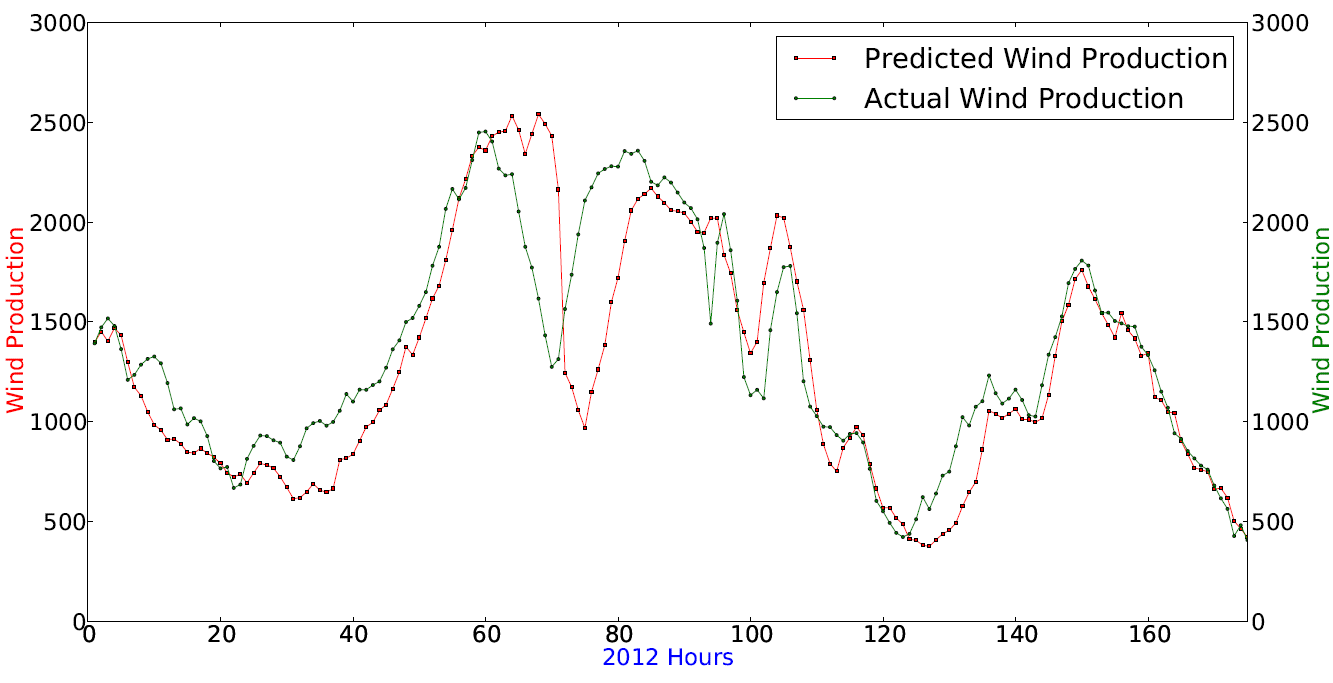
\includegraphics[width=0.99\linewidth]{billeder/curveAnalysisWindProduction.png}
\caption{Wind production prediction for 175 hours in 2012 with slope as input}
\label{fig:basicCurveAnalysisGraphoForDiscussion}
\end{figure}

It was expected to see better accuracy when applying calculated inputs to the electricity prices since it relies more heavily on previous prices and price movements in general as discussed in the price analysis in Section~\ref{sec:ElectricityPriceAnalysis}. Wind power follows meteorological factors more significantly which is expressed in the correlation to wind speed. The problem can be related to the electricity price being extremely volatile and the network not being able to identify a general recognizable pattern in how immediate hours impact the electricity prices when calculated (mentioned in Section~\ref{sec:usingStatisticalInput}).

The analysis establishes that previous hours impact the price and wind power but not if the actual skewness or historical volatility calculations have an influence. The reason is the many adjustable settings (see Section~\ref{sec:windProductionDev}) of the functions which in our opinion makes them more applicable for testing directly in experiments based on the conclusion that previous hours influence the output. What can be concluded from the results is the potential benefit from using calculated inputs to add additional characteristics about the movements of the curve and help the generalization function of the network to approach its target better --- if the correct calculated inputs are used. Alternative calculations from the field of economics could be investigated to include additional features and characteristics of the curve movements but also hybrid versions of the Artificial Neural Network can be studied. One such hybrid is a Wavelet Neural Network (WNN) where the properties of a wavelet is utilized in \cite{adaptiveWaveletANNElectricityMarkets} and the wavelet shape is adapted according to the training dataset instead of adapting the parameters of a fixed shape function (an example is the sigmoid function) by adjusting weights. Their point is that a WNN is better at generalizing high frequency signals than the Feedforward Neural Network that we are using here. It has not been considered in this thesis but based on the above description it potentially can improve the accuracy.

\subsection{Experiment four}
\label{sec:blackBoxDiscussion}
The purpose of the black box optimization was to find the best number of epochs and best size of the training set. It showed in both predictions --- wind power and electricity price --- what was expected of it. It revealed that too many or too few number of epochs resulted in an over- or under-fitting of the networks function. Section~\ref{sec:annSection} describes common pitfalls when using Artificial Neural Networks where the generalization function of the network is overfitted. In short the generalization function is fitted only to the training set and therefore not able to predict beyond it, i.e. predict the values in the testing set. In this thesis we have dealt with over-fitting by early stopping and dividing the datasets into a training set and a testing set. We tried different epochs from 1-2800 and selected the number of epochs that achieved the best result on the testing set. It gives the best picture since predictions will naturally be done on data that has not been seen before. 

Over- and under-training of the network as presented in\cite{1} was more clear for wind power. Too few  and too large datasets resulted in a significant worsening in the error from 19,7\% to 48,64\% compared to the best size of data at 3 month (Section~\ref{sec:experimentFourBlackBox}). The same did not apply for electricity prices where the best size showed to be half a year and where the errors were closer to the best result varying from 3,19\% to 7,19\% (Section~\ref{sec:priceExperimentFour}). It emphasizes the need for experimenting with the right amount for the specific type of prediction.

The purpose of the time measurements is to illustrate the impact of training set size on pruning, training and prediction. The prediction time showed to be almost linear with the training set size in both cases. The times varied from 232 to 844 seconds for electricity prices and 462 to 1585 seconds for wind power for predictions over an entire year. The difference between electricity price and wind power numbers is found in the use of two computers with different computational power. A time-consuming element in the predictions are the identification of the network structure through pruning and the actual training of the network before doing all day-ahead predictions --- this procedure is always done before the predictions. The beginning procedure accounts for about 1/20 of the time whereas the subsequent 360 predictions (one for each day of the year) is the rest. The best electricity price prediction took 397 seconds which would result in approximately 20 seconds (397/20) of pruning and training before being able to predict. The individual predictions take only seconds and in a real setting only one day is predicted at a time which makes the pruning and training the most significant time waste --- the approximately 20 seconds of wait time and the few seconds it takes to predict makes it possible to use the Artificial Neural Network model just before the time to predict. If time becomes an issue our results show the influence of computational power to be considerable and an increase could be used as a solution to bring down the time to predict. The focus on the time perspective would have another meaning if the algorithm was to be used in an autonomous trading system with the purpose of placing bids itself but this will not be discussed further.  

The best results from Section~\ref{sec:experimentFourBlackBox} and ~\ref{sec:priceExperimentFour} show how the results can be considered as robust and steady. The top five for wind power with differet epochs vary from 121,02-125,96. For price the top five goes from 45,17-47,92. It emphasizes that the inputs and their representation influence the wind power and electricity price as seen throughout the previous experiments.

Section~\ref{sec:experimentFourBlackBox} and ~\ref{sec:priceExperimentFour}

\subsection{Experiment five}
\label{sec:stepAheadForecastingDiscussion}
Experiment five was conducted because we saw that the system performance was directly related to number of hours (unseen data) it had to predict and where the offset for the prediction was set.
\subsection{Step-ahead forecasting}
\label{sec:stepAheadDiscussion}
The step-ahead experiments shows how each step are based on the step before it; because we include the last-known price (in the price predictions) and the last-known wind production(in the wind production predictions). When steps increase then the accuracy will decline thus introducing larger errors. This is because there is a certain elevation of error in our predictions because of the aforementioned last-known price and last-known wind production. In both of our results we see an improvement in the MAE with fewer hours to predict ahead. We also see that the elevation of the error at some point flattens thus not rising uncontrollably. This is because the other input parameters also influences the prediction (and not only the last-known price/wind production) thus guiding the prediction in the right direction. The step-ahead forecasts shows how important it is to use the predicted values and simulate a real life setting when doing the benchmarks for the specific dataset. If we did not use the predicted price when doing the next prediction in a 24 step-ahead forecast and if we instead used the exact value; then we would just be doing a 1 step-ahead forecast in 24 hour chunks. This again cements the need for transparency in what is done during a simulation to be able to reproduce the experiment but also be able to verify the results.

This is a place where we can improve our algorithms since the error margin introduced by x hours-ahead are significant. Future work in this area includes predicting the next hour several times and taking the average of this thus reducing the error of one faulty prediction. This should help the ANN to limit the elevation of the error. Another approach would be to include the predicted step into the dataset and train the network again including the newest prediction thus adjusting the weights to accommodate the most recent prediction. The future work also includes looking into ways of eliminating the last-known price as an input thus eliminating the source of the elevation in errors. This could include a scatter scheme similar to the one presented in \cite{singhal2011electricity}. The step-ahead predictions also verifies the need for the predictions to be done on unseen data (as described in Section \ref{sec:inputParameterDiscussion}) and the need for simulation of unknown prices during the 24 hours we want to predict. 
\todo{insert picture for 1 step-ahead and 24 step-ahead}

\subsection{Offsets}
\label{sec:offsetsDiscussion}
Another source of errors are the changing offsets in the predictions. When we (in the previous experiment) change the number of hours to be predicted ahead we also change the offsets used to predict from. Some of the offsets in the dataset are better starting points (for a prediction) than others - reflected in the Table \ref{table:stepAheadForecastingWindProductionStartingPositions} and in Table \ref{table:Offsets} with an improvement of 23,34\% and 15,04\% respectively. The offsets in the dataset are not something that is covered in other papers (that we have read) which demonstrates the need for an expressive data analysis/experiment section that clarifies what they know about the dataset and how the predictions are affected. We also see papers that only use 1-2 weeks\cite{yamin2004adaptive} or only days \cite{1, singhal2011electricity, pjmForecast} for their test datasets. These papers do not state anything about changing offsets or what time of day they begin the prediction. When they have relatively small testing datasets the error from the right offsets will be significant thus we see a need for addressing it. Jonsson et al.\cite{forecastingSpotPricesAccountingForWindPower} writes that they do predictions from midnight to midnight to resemble how day-ahead forecasts are done in practice. This point is valid but still does not account for the offset problem. As we discussed in Section \ref{sec:unseenDataDiscussion} the need for testing all the different possibilities are important to get a full picture of how well a solution predicts the prices. If a setup was to be used in a live setting the changing offsets should be considered when stating how well a system performs. Also if this is not stated clearly in papers we can only make assumptions about how they subject to these factors if they do at all. The offsets are also a place for improvement. In both experiments (Section \ref{sec:windPowerExperimentFive} and Section \ref{sec:priceExperimentFive}) the predictions are better if we start in the right offset. If we can analyze the best starting points and see what characteristics they have in common - then the right offset can be chosen before every day-ahead prediction.

\subsection{Artificial Neural Network for prediction}
\label{sec:annForPrediction}
This section will discuss the feasibility of Artificial Neural Network as a technology for prediction of electricity prices and wind power. The hypothesis presented in Section~\ref{sec:theHypothesis} and the experimental results will be the basis for the discussions. Following quotation from the hypothesis section has been pointed out:

\begin{quotation}
\textit{Artificial Neural Networks can be characterised as Machine Learning\cite{18} and therefore it must be trained with historical data that is relevant for the specific task. The goal is to investigate and identify (through analysis and experiments) the importance of the influential factors to be included and represented in these datasets. Based on this we examine the feasibility of a Back Propagation Artificial Neural Network as a technology for predicting electricity prices and wind power. The feasibility will be examined by analysing the experimental results and the potential for practical use.}
\end{quotation}

\noindent The hypotheses take its outset in how to utilize the Artificial Neural Network best possible by analysing the influential factors, representing them appropriately and verifying it through experiments. Answering the feasibility question regarding ANN as a proper technology for predicting electricity price and wind power will be based on these parameters and on its potential for decision making in practice. It will be structured in the following way:

\begin{itemize}
\item Input analysis and transparency: This section will be dealing with the importance of investigating the influential factors.
\item Trustworthiness: The section considers the conducted experiments to verify the analysis and how to trust them.
\item Feasibility: Will conclude on the feasibility based on \#1, \#2 and our experimental results.
\end{itemize}

\subsection{Input analysis and transparency}
Artificial Neural Networks as a technology for prediction in the electricity market is much dependent on the analysis and experiments surrounding it. The experiment discussions above highlight the need for analysing and documenting characteristics of what is to be predicted by the ANN. Machine Learning is data-driven\cite{18} and the analysis together with experiments point out the influential input parameters to include in the dataset that is the basis for the data-driven learning. The analysis will identify the input parameters to test and the experiments will either reject or verify what came out of the analysis. The result will be the best network setting along with a common understanding of exactly why these input parameters did the job for this market and why others did not. In continuation of this lies the need for transparency when using ANNs since omitting it will make it difficult to draw on the experience of others and make comparisons between systems due to the black box nature of the technology. Comparisons are possible if both attempted to predict the exact same market and used the exact same performance measure. The need for transparency becomes even clearer when the ANN is supposed to used in practice according to Section~\ref{sec:annForDecisionMaking}. 

In Section~\ref{sec:inputParameterDiscussion} we discuss the difference in experimental setups from publication to publication and how it becomes difficult to imitate when the information about it is incomplete. Based on discussions throughout the thesis and the comparison conducted in the experiment from Section~\ref{sec:priceExperimentThree} we argue that such comparisons are not even fair due to the lack of documentation regarding input analysis, dataset and experiments. An example of a meaningful price parameter in the Danish electricity market which does not apply for all markets is wind speed due to the large amount of wind mills in Denmark. This parameter shows a co-relation of 0,28 (Section~\ref{sec:Price}) and it is clear from the analysis why it has been included in the experiments where the influence is verified even to a greater extend than expected --- predicting the prices in a country without many wind mills should probably not expect the same benefits when using our setup with wind speed which should be apparent from the analysis in Section~\ref{sec:priceWeatherInfluence}. Another example exist for wind power where demand is analysed to greatly influence the production but is instead substituted with air density in the best prediction due to air density being calculated with temperature and pressure. Temperature highly influences demand and because pressure is close to constant the air density express temperature (see Section~\ref{sec:predictionBasicInputParams}). Dataset manipulation can greatly affect the predictions as well as discussed in Section \ref{sec:matrixTrimmingDiscussion}. Matrix representation of the input parameters proved to affect both datasets positively. The trimming only improved the price predictions but with a substantial improvement. If not documented properly the use of these input parameters and dataset manipulations are unclear and it would require investigation and assumptions by others to replicate. The overall benefits obtained in our experiments will most likely \emph{not} be the same when used in markets with different properties. It emphasizes what have been said earlier, namely that transparency in an analysis is necessary to make comparisons and knowledge sharing possible but at the same time to identify the best possible setting yourself. The feasibility of the ANN should not be judged on its results alone (MAE, MAPE) but also on how and why the input parameters were selected and represented in the dataset. Both because what makes it applicable in one setting does not necessarily apply for another but also because we need to trust that the dataset is selected and tested based on a satisfactory foundation --- the resulting error can best be explained by looking at exactly what conditions constituted it. For instance, all our prediction experiments use last hours production or price as input and the accuracy will drop significantly if the day-ahead forecast uses the predicted value (which is the case for this thesis because it mimics real use) instead of the ideal. This is discussed in Section~\ref{sec:stepAheadForecastingDiscussion} but the point is that this information is necessary to have any idea of the result. This leads to the trustworthiness of a system in terms of the experiments performed to verify the inputs which will be the topic of the next section.  
\todo{we could have been more structured --> trend analysis and statistics}

\subsection{Trustworthiness}
A reliable prediction must have included all the right input parameters based on a comprehensive analysis in combination with a series of experiments that validate the findings. Section~\ref{sec:unseenDataDiscussion} emphasize and discuss the necessity of simulating predictions for at least a year to strengthen results. The year contains many different days and the seasons have different conditions, e.g. winter calls for heating and a lot of indoor activity whereas the summer is equal to holiday and being outdoor which is obviously reflected in the prices seen in Section~\ref{sec:seasonality}. The changes are also apparent for wind power but mostly due to the changes in weather conditions during the year (see Section~\ref{sec:windProdSeasonality}). The wind power seasonality is shown in graphs from Section~\ref{sec:windPowerBestPredictionGraphs} where spring and fall have been highlighted in Figure~\ref{fig:bestWPPredictSpringForDiscussion} and~\ref{fig:bestPredictWPFallForDiscussion} (the difference between the two should be apparent). We have shown examples of articles predicting only individual days or weeks and argue it to be sufficient (discussed in Section~\ref{sec:inputParameterDiscussion}). We consider it necessary to simulate the predictions for an entire year in all experiments so that all conditional changes of every season are included and reflected in the results --- this is of course time-consuming but argued to be necessary. Besides from the impact of different seasons our results showed a great variation in error according to the starting point of the prediction. It emphasizes how different scenarios have different results and therefore must be covered during testing. The discussion is elaborated in Section~\ref{sec:stepAheadForecastingDiscussion} where the potential elevated error depends highly on the starting point of the prediction. The trustworthiness of the prediction is related to how thoroughly it has been tested and how many scenarios have been covered to simulate the greater part of possible use cases. 

\begin{figure}[H]
\centering
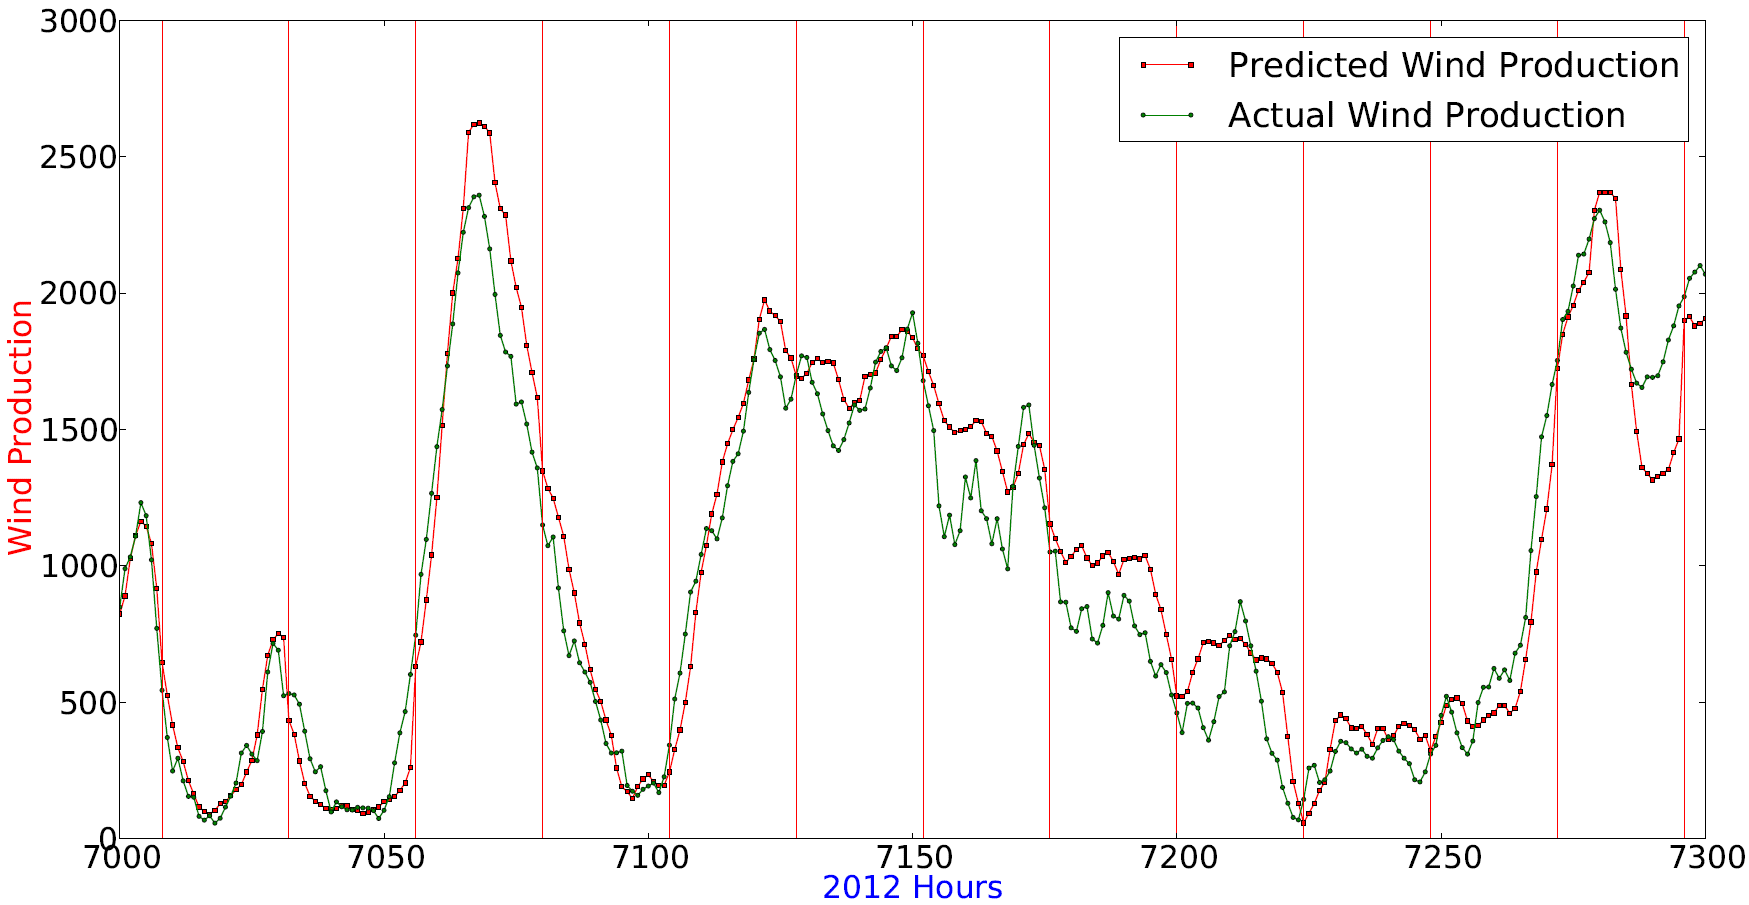
\includegraphics[width=0.99\linewidth]{billeder/bestPossiblePredictionWindProduction7000-7300_Fall.png}
\caption{Best prediction for 300 hours for Oct-Nov (Fall)}
\label{fig:bestPredictWPFallForDiscussion}
\end{figure}

\begin{figure}[H]
\centering
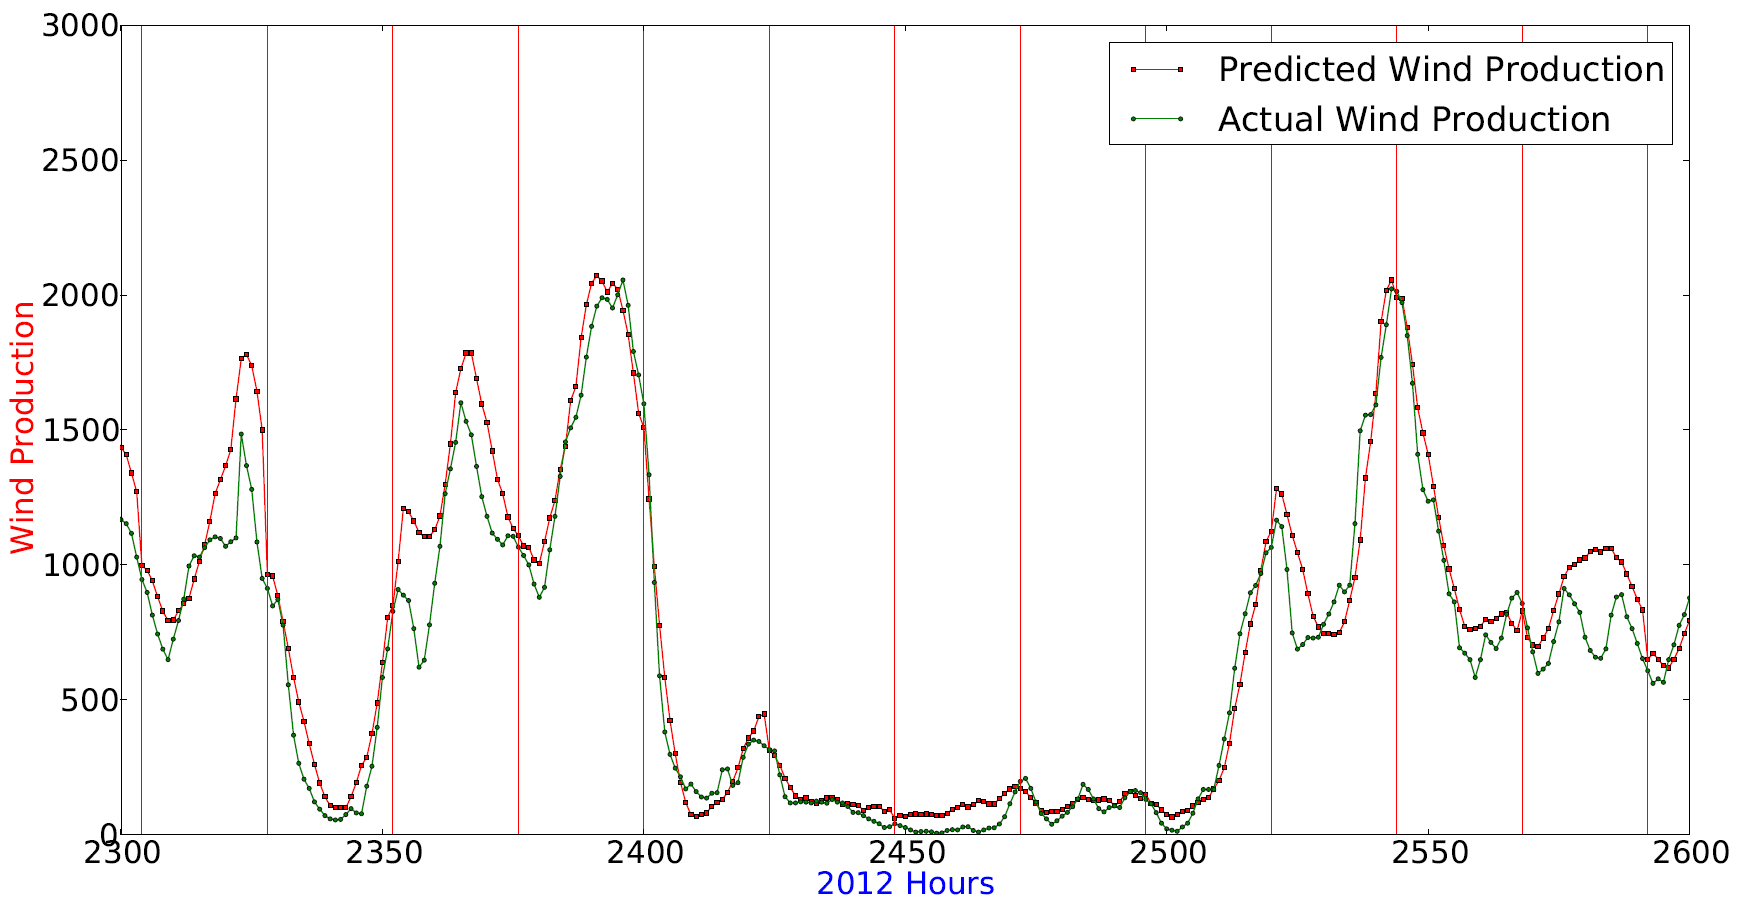
\includegraphics[width=0.99\linewidth]{billeder/bestPossiblePredictionWindProduction2300-2600_April_Spring.png}
\caption{Best prediction for 300 hours of April (Spring)}
\label{fig:bestWPPredictSpringForDiscussion}
\end{figure}

When arguing the need for testing on an entire year we must highlight the different results when running the same prediction again (discussed in detail in Section~\ref{sec:unseenDataDiscussion}). In our thesis we use an entire year to cover all conditions during a year as well as predicting similar days more than once. An alternative could be to run the yearly experiments more than once and deliver the average error for all test runs. This would strengthen the results but must be a trade-off between time constraints and trying to cover most cases (exemplified in Section~\ref{sec:windPowerBestPredictionGraphs}). Another impact from our dataset could be the fact that our testing set does not contain any predicted values. This can negatively affect the predictions when used in a real life setting and testing of this must be included in future work. We still consider the actual values to be sufficient since they look exactly the same and can simulate the predicted values in our experiments (simulation of a real setting). Furthermore, it gives us the opportunity to simulate all possible predictions of an entire year (since historical prediction data is not available to our knowledge) which our experiments show the importance of as described above. The analysis of the actual values show what influence the electricity price and wind power and in future work we must rely on other professionals to give us the best possible predictions of consumption and weather so that they are accurate enough to be consistent with the analysis. The weather predictions will deviate from the analysis \emph{only} if they are inconsistent and inaccurate but as described in Section~\ref{sec:dataCollection} the accuracy of 24 hours weather prediction is 97\%. We consider the results obtained in this thesis valid because the potential decrease in accuracy would apply for all results, highly ranked or not. It correctly shows the co-relation between input/output, the ranking of results and the input combinations used. It must be pointed out that the results are not definitive but gives a clear indication of the influences of wind power and electricity prices as well as showing what data manipulations work for the Danish electricity market. The transparency of an Artificial Neural Network and its black box is considered a key to the feasibility of the predictions themselves because it implies trustworthiness. Transparency becomes of even greater importance when applying the ANN in a real setting for decision making --- will be discussed next.

\subsection{Feasibility}
The feasibility of the Artificial Neural Networks as a proper technology for prediction will be based on conclusions from the discussions just above, the experimental results and its potential for being used in practice. Results will not be compared to other Artificial Neural Networks since it has been found out of scope and even unfair. Early discussions showed how comparisons between ANNs require rebuilding and imitation of the experimental setups and then running it on our own datasets. This can be very difficult and even meaningless due to different market conditions and incomplete analysis and documentation. We made an example by attempting it in Section~\ref{sec:priceExperimentThree} where our own approach obtained 11\% better MAE than the other on our dataset. Without any prober analysis of their market, dataset and experimental setup we have no foundation for making any assumptions of their resulting error. We can conclude that with the information we were able to extract it did not work for the Danish electricity market. Section~\ref{sec:influenceOfTrendInCalcInput} presents a publication that forecasts electricity spot prices for Western Denmark (DK-1) from Nord Pool Spot. Their results have been used to position our approach and determine the feasibility of our experimental results. We achieved 34 DKK better MAE than the simplest approach, 2 and 4 DKK worse than their ARIMA and Holt-Winters approach and 11 DKK worse than their best approach. The results are not definitive but can be used as an indicator for the Artificial Neural Networks ability to predict electricity prices for western Denmark. Furthermore they present the Wavelet Neural Network as a technology that most likely can obtain similar results to their best approach which could be explored further in future work.

The feasibility of the proposed ANN can be seen as a direct result of the identified input parameters and their representation. The analysis, the actual selection of inputs and the experiments is what constitutes the prediction and explains the obtained experimental results --- it is also what creates trustworthiness in the results (MAE, MAPE). The prediction is data-driven and as a result no better than the dataset it is trained upon. The feasibility should therefore be mentioned based on the analysis of input parameters and how they were validated through experiments. This of course presupposes that the prediction experiments must cover as many scenarios as possible. Days are different and the overall feasibility of the ANN is not conveyed if not tested on a satisfactory amount of data. We argue that the final prediction error cannot stand alone without a description of exactly what constituted it and why. We have in this thesis satisfied the above by a thorough analysis of the influential factors for electricity price and wind power for Western Denmark in Chapter~\ref{ch:theANNs} which have been validated through various experiments performed on an entire year in Chapter~\ref{ch:experimentalResults}. The experimental results show how the predictions evolve from experiment to experiment and how the different strategies affect the prediction results which is in agreement with our original purpose, i.e. to investigate and identify the importance of influential factors to be included and represented in the dataset. The best result for wind power misses its target by 121,02 MWh out of the interval from 0-2753 which corresponds to 4,4\% of the 2753 possible values. The influential factors was wind speed, temperature, last known wind power, time of day and historical volatility. The best electricity price prediction achieved 45,11 DKK out the interval of 61-632 which corresponds to 7,9\% out of 571 values (632-61) on demand, wind speed, temperature, time of day, time of week, season of year, skewness and historical volatility. Examples of the predictions can be seen for wind power in Figure~\ref{fig:abilityToPredictWindPower} and for the electricity price in Figure~\ref{fig:abilityToPredictElectricityPrice} --- the graphs are taken from Section~\ref{sec:windPowerBestPredictionGraphs} and ~\ref{sec:priceExperimentFour}. The most striking thing from the graphs is the difference in volatility which makes the electricity price harder to predict (which has also been stated throughout the analysis and experiments).

\begin{figure}[H]
\centering
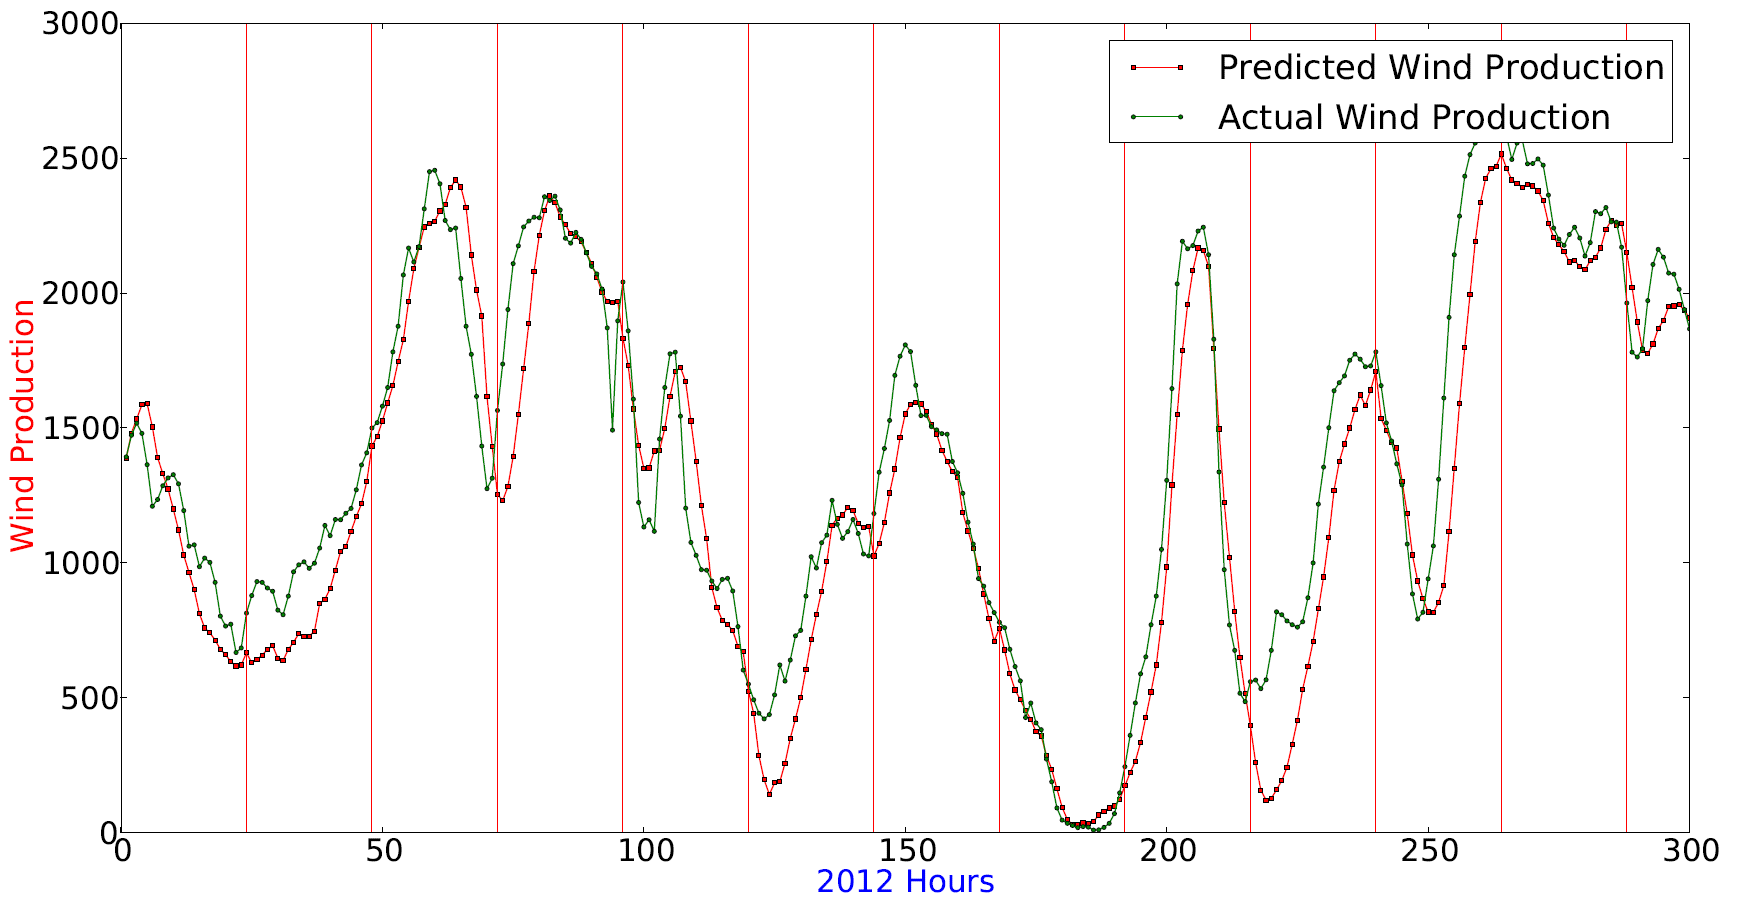
\includegraphics[width=0.99\linewidth]{billeder/bestPossiblePredictionWindProduction0-300.png}
\caption{Wind Power best prediction for 300 hours of January (Winter)}
\label{fig:abilityToPredictWindPower}
\end{figure}

\begin{figure}[H]
\centering
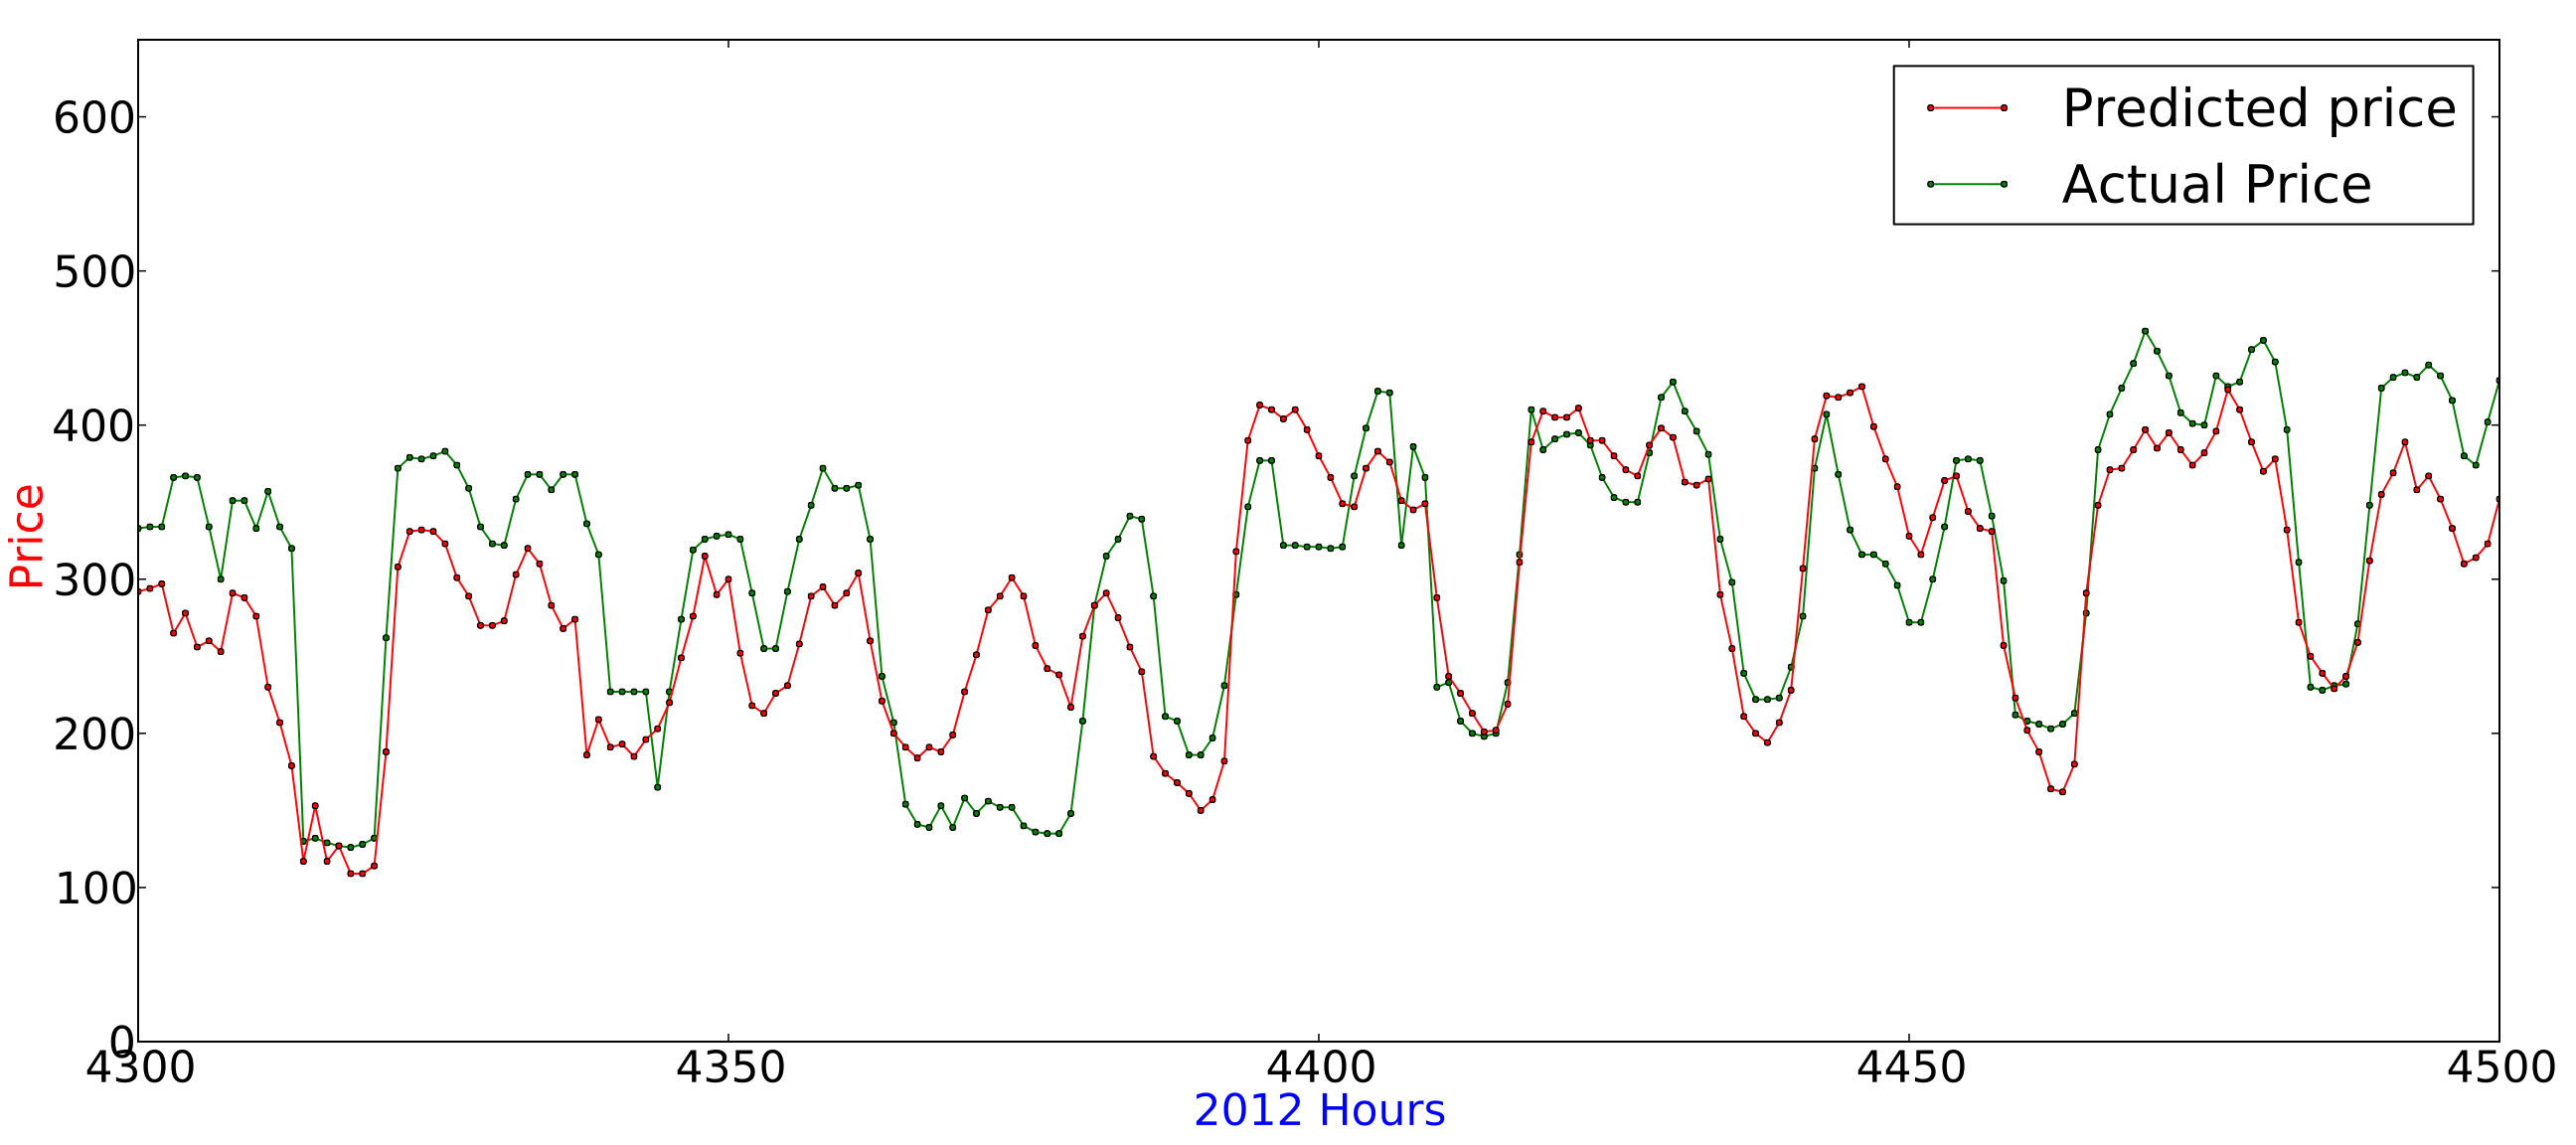
\includegraphics[width=\linewidth]{billeder/PriceExperimentalAnalysis/summer.jpg}
\caption{Electricity price on 200 hours from summer}
\label{fig:abilityToPredictElectricityPrice}
\end{figure}

We have attempted to simulate real use in our experiments by predicting day-ahead prices and wind power productions over a whole year with different offsets where every predicted hour uses the last predicted hour (except from the first hour) which indicates that our modelled ANN can be used in practice. The preconditions and challenges for using ANN in practice has been discussed in Section~\ref{sec:annForDecisionMaking} where the general theme is transparency and how it also can be used to ensure trustworthiness in the context of a Decision Support System. Ensuring trust in a prediction is of utmost importance when basing a decision on it and therefore issues that have been discussed here can be transferred to this specific purpose --- especially the need for analysing and bringing forward the underlying data used for predicting the electricity price or wind power in order to create trust.
 
\subsubsection{Concluding Remarks on Feasibility}
The above discussions comply well with the fact that machine learning is not all technical bot also intuition, creativity and black art\cite{18}. For instance a great deal of intuition and creativity goes into designing the experiments. Everything cannot be tested and you must rely on intuition to include all situations necessary for testing, and the creativity resides in how to actually do it. Furthermore, the different inputs can be represented in various ways that calls for creativity --- represent input as a matrix, calculate slope or volatility and represent the seasonal aspect as month or summer/winter/spring/fall. The ANN being black art or a black box requires intuition in itself since we cannot foresee the outcome. When analysing prediction results from the experiments we rely on the analysis but also our intuition, especially in cases where things are not as we expected. We must assume based on the analysis and our intuition that this was what happened. It is again an argument for analysis and experiments to be documented for both own benefit and the sake of transparency for others. The following points sum up the above discussions regarding feasibility of the Artificial Neural Network.

\begin{itemize}
\item We have analysed the influential factors of wind power and electricity prices in western Denmark and verified the best combination through experiments. It has been shown that the feasibility of predictions that originate from an ANN is highly connected to performing a proper analysis and testing it which has been done in this thesis. Furthermore, the need for transparency was highlighted in this context to ensure both trust but also for others to see feasibility in the predictions that use ANN as technology.
\item Strategies have been applied in an attempt to improve accuracy (data manipulation, matrix, black box). We have shown how they can be applied to the inputs and has shown an improvement in accuracy throughout the experiments. The ANN for prediction can be significantly improved by manipulating the dataset to fit the problem and increase its potential accuracy.
\item The experiments must be performed on a satisfying number of days on an unseen testing set. We suggest a year so that most cases are covered in order for the ANN to show its potential in a realistic setup --- this setup convey the potential for practical use due the simulation of many different scenarios during the year. 
\item We see the feasibility of the ANN as directly linked to its potential for practical use which the experiments speak in favour of by covering many possible use cases. In this regard the transparency in underlying data must again be highlighted because it is equally important for creating trustworthiness in practice due to the chaotic behaviour of the electricity price and wind power. It puts even more emphasis on the need for properly analysing and experimenting so that it can be both taken advantage of when ensuring the feasibility of both model and practical use. They both rely great on it.  
\end{itemize}

\subsection{Artificial Neural Network for decision making}

\subsection{Future work}
this section will discuss what can be done in relation to strategies or other attempts to improve accuracy of the predictions.

\subsubsection{Recalculate}
POTENTIAL STRATEGY
The re-calculation concept works by letting other neural networks re-calculate the prediction from the original network. The purpose is to identify places where the generalization function has problems and then divide it into new neural networks that only have the purpose of focusing on these problematic situations. For simplicity we are going to apply this to the small numbers and big numbers of the dataset. We will define what is small and big by taking the 2 and 98 percentile. Whenever the "original" network predicts something in or close to the big or small interval then the responsibility of that prediction is forwarded to one of the two. It works like a second opinion but here the network has been specialized to only focus on a specific part of the dataset instead of everything\todo{give example of corrections}. It creates a normalization function on a smaller dataset and the idea is to leave out a lot of unnecessary information. It does not need to account for anything other than its interval in the generalization function so it should be able to predict its target group better. We let the original network decide if it actually thinks we are in the low numbers --- if we are then we can possibly make that prediction even more accurate. These thoughts could basically we applied on all other parts of possible wind production values. 

Problem can occur if the intervals are too small which will cause the dataset to be too small and hard for the ANN to generalize upon.

\subsubsection{Prediction - Similar Days}
The similar days approach is described in Section~\ref{sec:sdmApproach} and addresses what to include in the dataset based on parameters. Wind power production follows wind speed and the expectation is that if filtering out days with completely different wind speeds and productions then a better accuracy can be obtained. The similar days analysis will take all wind speeds from the hours to predict and find all days within this interval plus/minus one in each end, e.g. an interval of wind speeds between 4-9 would result in similar days between 3-10. There is a potential for not getting the entire picture when using similar days. It can be related to the discussion about wind speed as matrix and how some values are under-represented in the dataset. In could happens in shifting seasons that wind speeds are never seen before and therefore run into a dataset without many hours. In those cases the entire dataset is used instead. The analysis in Section~\ref{sec:windProdSeasonality} describes the difference from season to season.

We can see from Table~\ref{table:theSimilarDaysApproach3monthTable} that the results are much equal to the best input combination from Table~\ref{table:windProdInputParamsTop10}. The purpose of the similar days is to filter out unnecessary noise from the dataset but since the dataset is of a manageable size and in itself contain a seasonal aspect it does not filter out many values as seen in the table. When applying it on an entire year more values are filtered out but it cannot make up for the increase in dataset as seen in Table~\ref{table:theSimilarDaysApproachYearTable}.

\todo{USE THE MODEL FROM UNCERTAIN INFORMATION}

\todo{discuss how the two predictions are related which is seen by the connection between wind speed and price and the 'Day-Ahead Electricity Prices in Denmark: The Impact for Wind Power Forecasts}

\todo{discusss why wind power production variations (as described in the introduction) was not used in electricity price}

\todo{relate to why we can do this without expert help but the next step to integrate a fully working dss would require expert to know what to do configurable}

\todo{why analyse? First of all in order to identify parameters but also so that other can build on your experience in a field that is so hard to do comparisons in}